\documentclass[12pt]{tehranReport}
\usepackage{ptext}
\usepackage{hyperref}
\usepackage[framed,numbered,autolinebreaks,useliterate]{mcode}
\usepackage{graphicx}
\usepackage{subcaption}
\usepackage{relsize}
\usepackage{mathtools}  
\usepackage{diffcoeff}
\usepackage{mathrsfs}
\usepackage{multirow}
\usepackage{algorithm}
\usepackage{amsmath,amssymb}
\usepackage{algorithmic}
\usepackage{xfrac}  
\usepackage{xepersian}


\title{موضوع}
\author{نام دانشجو}
\authorPosition{}
\university{دانشگاه تهران}
\college{پردیس دانشکده‌های فنی\\دانشکدهٔ برق و کامپیوتر}
\studentNumber{شماره دانشجویی}
\course{نام درس}
\supervisor{نام استاد}
\settextfont[Path={./font/}, BoldFont={XB NiloofarBd.ttf}, BoldItalicFont={XB NiloofarBdIt.ttf}, ItalicFont={XB NiloofarIt.ttf}]{XB Niloofar.ttf}

\begin{document}

\maketitlepage

\tableofcontents
\newpage
\renewcommand{\thesection}{\arabic{section}}
\section*{چکیده}
بخش چکیده 
\newpage
\section{تجزیه مقدار تکین }
تجزیه SVD در جبر خطی, نوعی تجزیه است که در آن یک ماتریس حقیقی یا مختلط را به ضرب یک ماتریس قطری با 2 ماتریس مربعی که با پایه های بردار ویژه بدست می آید, تبدیل می کند. این تجزیه سیستم را به ترکیب خطی عناصر مستقل تبدیل می کند که هر کدام از آنها سهم خود را از انرژی کل سیستم دارند.
برای مثال در تجزیه یک ماتریس $M \times N$ داریم:(با فرض $M \geq N$)
\begin{figure}[h!]
	\centering
	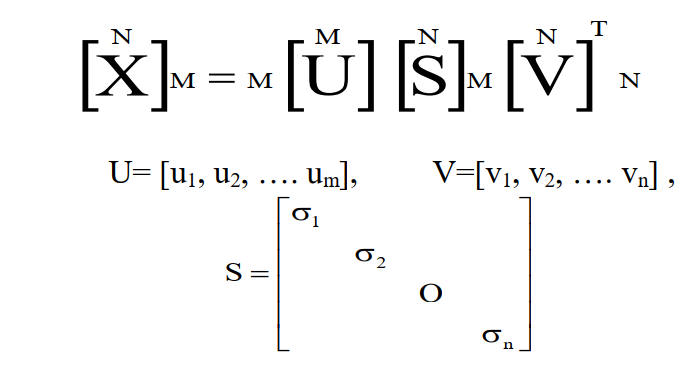
\includegraphics[width=\linewidth, height=0.3\textheight]{pics/1}
\end{figure}\\
ماتریس S قطری است که مقادیر ویژه ماتریس X بصورت  نزولی در قطر آن قرار گرفته اند. ماتریس U با تبدیل بردار های ویژه $X X^T$ به بردار هایی یکه و تشکیل آن ها به صورت 
$$
U = \begin{bmatrix}
	u_1 && u_2 && ... && u_m
\end{bmatrix}
$$ 
که $u_i$ نشان دهنده بردار ویژه یکه $i$ ام است, بدست می آید. به همین صورت با بدست آوردن بردار های ویژه ماتریس $X^T X$ بردار V قابل بدست آوردن است. ستون های ماتریس متعامد U را, بردار های تکین سمت چپ و به همین صورت ستون های ماتریس متعامد V را, بردار های تکین سمت راست می نامند.
\newpage
\section{\lr{SVD-BASED ORTHOGONAL SUBSPACES AND RANK
		APPROXIMATION}}
همانطور که اشاره شد, یکی از کاربرد های مهم SVD, تجزیه ماتریس به ترکیب های متعامد است. معمولا بزرگترین اشیا در تصویر متناظر با مقادیر ویژه بزرگ و نویز های تصویر متناظر با کوچکترین مقادیر ویژه هستند. پس می توانیم داده ها را به ترکیب سیگنال و نویز تجزیه کرده و تخمین بهینه ارائه دهی. ویژگی اخیر می تواند در جهت فیلتر کردن نویز و فشرده سازی و حتی در شناسایی, به کمک اضافه کردن نویز مناسب به سیگنال به کار رود.
\\\\
	در تجزیه SVD رتبه ماتریس X برابر با تعداد عناصر غیر صفر در ماتریس قطری S می باشند. تصویر زیر را در نظر بگیرید:
	\begin{figure}[h!]
		\centering
		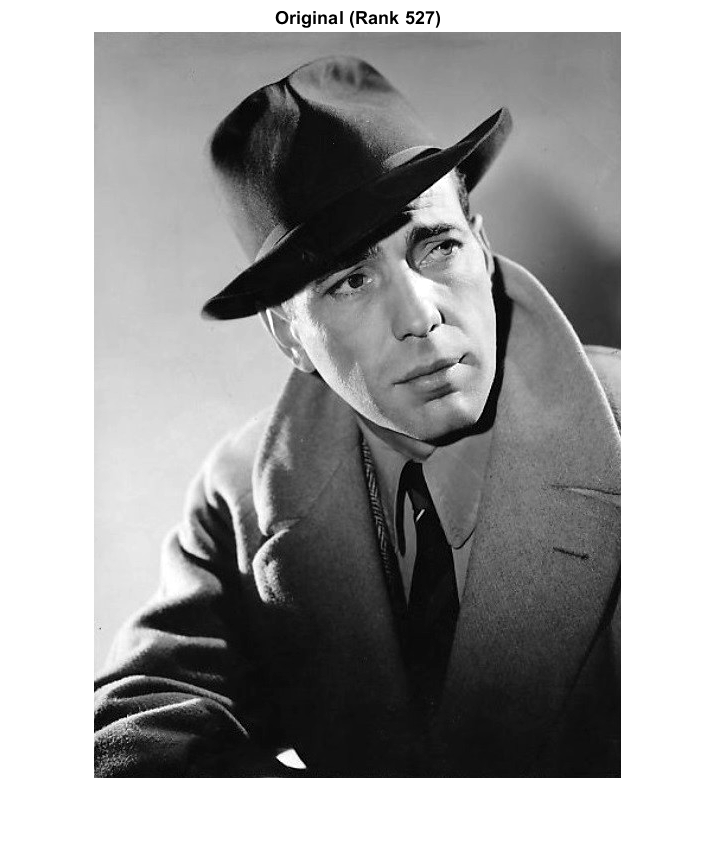
\includegraphics[width=\linewidth, height=.35\textheight,keepaspectratio]{pics/3}
		\caption{ عکس نمونه بدون فشرده سازی}
	\end{figure}\\
	از رابطه زیر که می توان یک ماتریس رتبه r را به r ماتریس رتبه 1 تبدیل کرد استفاده می کنیم.
	\begin{figure}[h!]
		\centering
		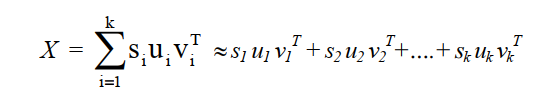
\includegraphics[width=.8\linewidth, height=\textheight,keepaspectratio]{pics/8}
	\end{figure}
	\newpage
	اگر در متلب تجزیه SVD ماتریس را محاسبه کنیم توزیع مقادیر وِیژه این تصویر به شرح زیر است:
	\begin{figure}[h!]
		\centering
		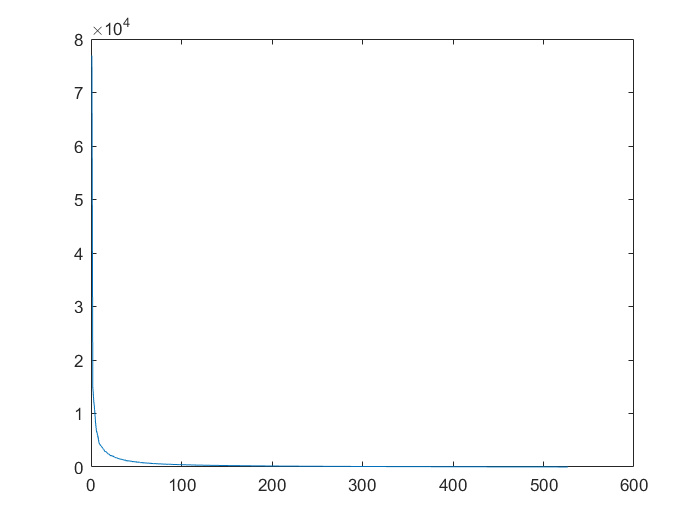
\includegraphics[width=\linewidth, height=.3\textheight,keepaspectratio]{pics/2}
		\caption{ توزیع مقادیر ویژه تصویر}
	\end{figure}\\
	همانطور که شکل 2 نشان می دهد اگر رتبه تصویر را تا مرتبه کوچک تری تقریب بزنیم, می توانیم بدون از دست دادن کیفیت بصورتی که توسط چشم قابل تشخیص باشد حجم تصویر را کم  کنیم. در شکل 4 این آزمایش را به صورت عملی انچام داده و نتیجه را مشاهده می کنیم.
	\newpage
	\begin{figure}[h!]
		\begin{subfigure}{.55\textwidth}
			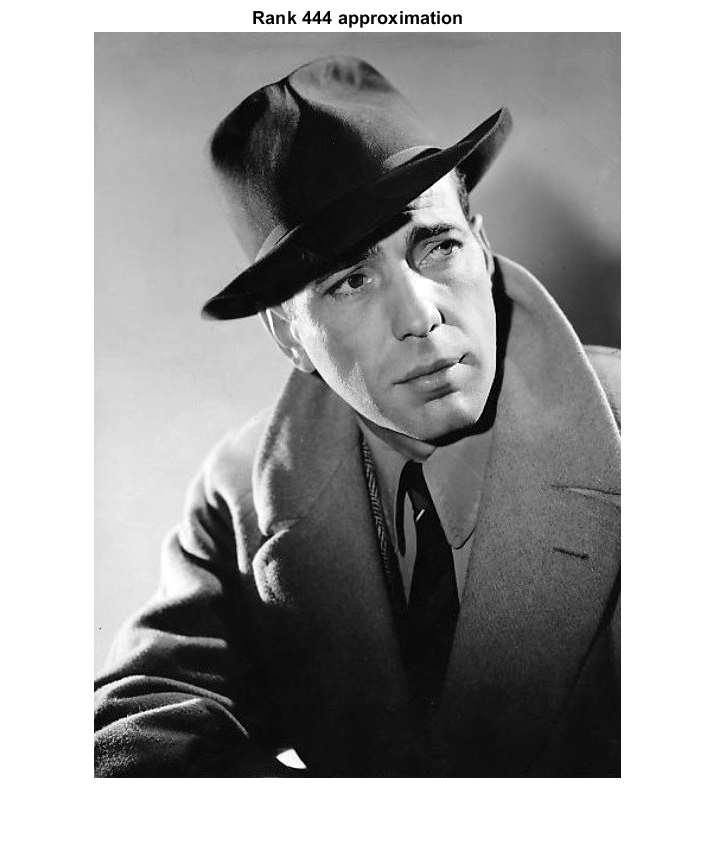
\includegraphics[width=\linewidth, height=\textheight,keepaspectratio]{pics/4}
			\label{fig:sub1}
		\end{subfigure}%
		\begin{subfigure}{.55\textwidth}
			\centering
			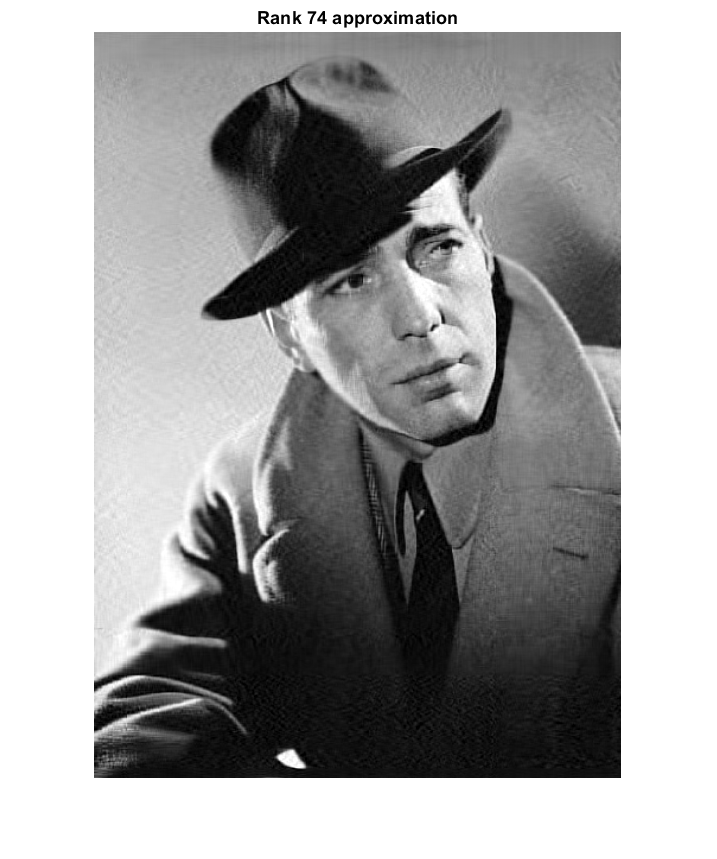
\includegraphics[width=\linewidth, height=\textheight,keepaspectratio]{pics/5}
			\label{fig:sub2}
		\end{subfigure}
		\begin{subfigure}{.55\textwidth}
			\centering
			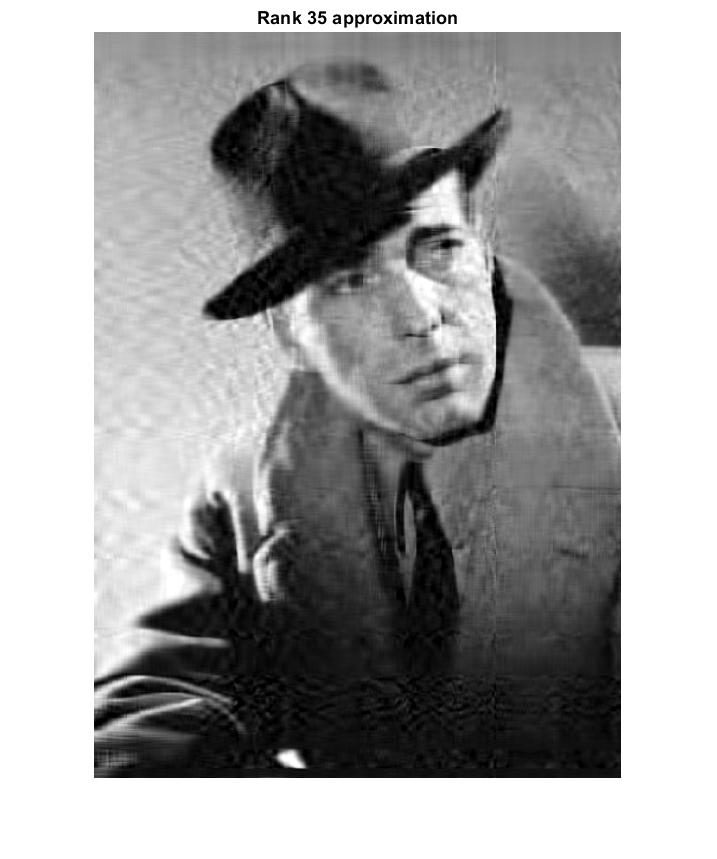
\includegraphics[width=\linewidth, height=\textheight,keepaspectratio]{pics/6}
			\label{fig:sub2}
		\end{subfigure}
		\begin{subfigure}{.55\textwidth}
			\centering
			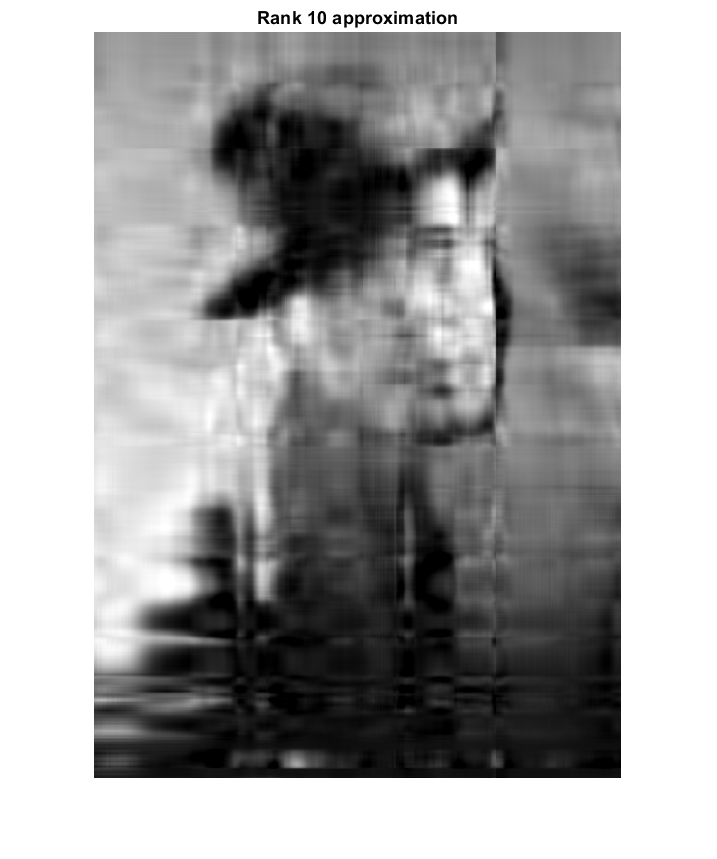
\includegraphics[width=\linewidth, height=\textheight,keepaspectratio]{pics/7}
			\label{fig:sub2}
		\end{subfigure}
		\caption{تقریب تصویر تا مرتبه های متفاوت و عکس حاصل شده}
		\label{fig:test}
	\end{figure}

\end{document}